% Fig. 1. Three panels stacked top to bottom, one column wide. Panels (a) and (b) are grey,
% panel (c) is in colour, and red marks only the words "link abstraction". The insets are
% schematic: (a) quality against SNR as a step, (b) as a smooth curve, (c) predicted against
% decoded quality along the diagonal.
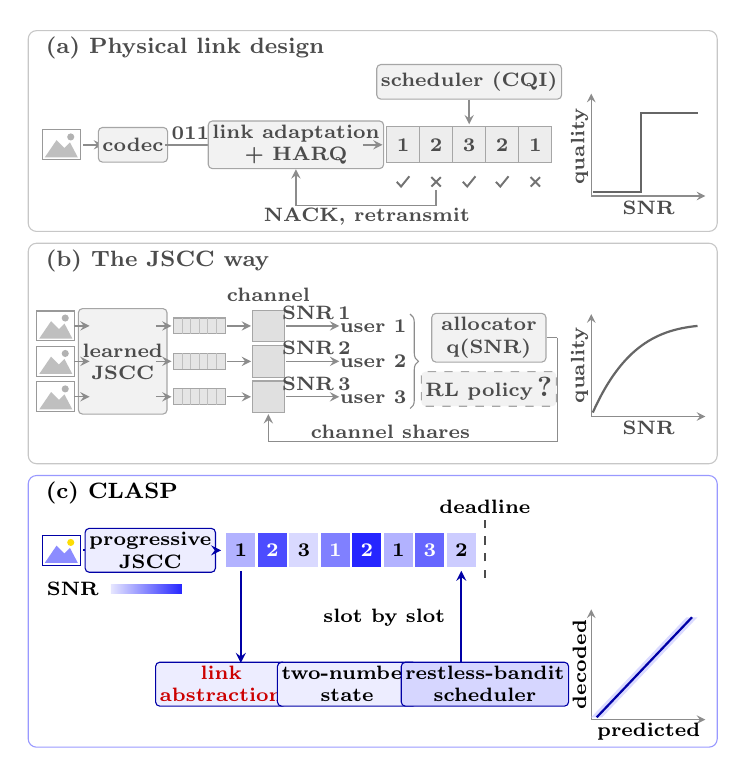
\begin{tikzpicture}[x=1cm, y=1cm, font=\footnotesize\bfseries, >=stealth,
  frame/.style={draw=black!22, rounded corners=3pt, line width=0.4pt},
  gbox/.style={draw=black!35, fill=black!5, text=black!70, rounded corners=1.5pt, align=center,
    inner sep=1.5pt, minimum height=0.44cm, font=\scriptsize\bfseries},
  cbox/.style={draw=blue!65!black, fill=blue!7, text=black, rounded corners=1.5pt, align=center,
    inner sep=1.5pt, minimum height=0.44cm, font=\scriptsize\bfseries},
  garr/.style={->, draw=black!45, line width=0.5pt},
  carr/.style={->, draw=blue!65!black, line width=0.6pt},
  gtxt/.style={text=black!70},
  small/.style={font=\scriptsize\bfseries},
  pics/gimg/.style={code={
    \draw[black!40, fill=white] (-0.24,-0.19) rectangle (0.24,0.19);
    \fill[black!25] (-0.21,-0.16) -- (-0.06,0.06) -- (0.04,-0.04) -- (0.11,0.03) -- (0.21,-0.16)
      -- cycle;
    \fill[black!30] (0.12,0.1) circle (0.045);}},
  pics/cimg/.style={code={
    \draw[blue!65!black, fill=white] (-0.24,-0.19) rectangle (0.24,0.19);
    \fill[blue!45] (-0.21,-0.16) -- (-0.06,0.06) -- (0.04,-0.04) -- (0.11,0.03) -- (0.21,-0.16)
      -- cycle;
    \fill[yellow!80!orange] (0.12,0.1) circle (0.045);}},
  pics/ok/.style={code={\draw[line width=0.7pt] (-0.08,0) -- (-0.025,-0.06) -- (0.08,0.07);}},
  pics/no/.style={code={\draw[line width=0.7pt] (-0.06,-0.06) -- (0.06,0.06)
    (-0.06,0.06) -- (0.06,-0.06);}},
]
% ---------------------------------------------------------------- (a) physical link design
\begin{scope}[yshift=0.5cm]
\draw[frame] (0,6.05) rectangle (8.75,8.6);
\node[anchor=west, gtxt] at (0.1,8.38) {(a) Physical link design};
\pic at (0.42,7.15) {gimg};
\draw[garr] (0.7,7.15) -- (0.95,7.15);
\node[gbox, minimum width=0.75cm] at (1.33,7.15) {codec};
\draw[garr] (1.74,7.15) -- (2.55,7.15);
\node[gtxt, small] at (2.14,7.3) {0110};
\node[gbox, minimum width=1.6cm] at (3.4,7.15) {link adaptation\\+ HARQ};
\draw[garr] (4.25,7.15) -- (4.5,7.15);
\foreach \i/\u in {0/1, 1/2, 2/3, 3/2, 4/1} {
  \draw[black!35, fill=black!7] (4.55+0.42*\i,6.92) rectangle (4.97+0.42*\i,7.38);
  \node[gtxt, small] at (4.76+0.42*\i,7.15) {\u};
}
\foreach \i in {0, 2, 3} \pic[black!55] at (4.76+0.42*\i,6.68) {ok};
\foreach \i in {1, 4} \pic[black!55] at (4.76+0.42*\i,6.68) {no};
\draw[garr] (5.18,6.57) |- (3.4,6.38) -- (3.4,6.84);
\node[gtxt, small] at (4.3,6.24) {NACK, retransmit};
\node[gbox, minimum width=2.1cm] (sa) at (5.6,7.95) {scheduler (CQI)};
\draw[garr] (sa.south) -- (5.6,7.41);
\draw[black!45, ->] (7.15,6.5) -- (8.6,6.5);
\draw[black!45, ->] (7.15,6.5) -- (7.15,7.8);
\draw[black!60, line width=0.8pt] (7.17,6.55) -- (7.78,6.55) -- (7.78,7.55) -- (8.5,7.55);
\node[gtxt, small] at (7.88,6.35) {SNR};
\node[gtxt, small, rotate=90] at (7.0,7.13) {quality};
\end{scope}
% ---------------------------------------------------------------- (b) the JSCC way
\draw[frame] (0,3.6) rectangle (8.75,6.4);
\node[anchor=west, gtxt] at (0.1,6.18) {(b) The JSCC way};
\node[gbox, minimum width=0.8cm, minimum height=1.34cm] (jscc) at (1.2,4.9) {learned\\JSCC};
\node[gtxt, small] at (3.05,5.75) {channel};
\foreach \k/\y in {1/5.35, 2/4.9, 3/4.45} {
  \begin{scope}[shift={(0.35,\y)}, scale=0.75] \pic {gimg}; \end{scope}
  \draw[garr] (0.58,\y) -- (0.78,\y);
  \draw[garr] (1.62,\y) -- (1.82,\y);
  \draw[black!35, fill=black!10] (1.85,\y-0.1) rectangle (2.5,\y+0.1);
  \foreach \t in {1,...,5} \draw[black!25] (1.85+0.108*\t,\y-0.1) -- (1.85+0.108*\t,\y+0.1);
  \draw[garr] (2.53,\y) -- (2.83,\y);
  \draw[black!35, fill=black!12] (2.85,\y-0.2) rectangle (3.25,\y+0.2);
  \draw[garr] (3.28,\y) -- (3.95,\y);
  \node[gtxt, small, above] at (3.66,\y-0.04) {SNR\,\k};
  \node[gtxt, small] at (4.38,\y) {user \k};
}
\draw[black!45, decorate, decoration={brace, amplitude=3pt}] (4.85,5.5) -- (4.85,4.3);
\node[gbox, minimum width=1.45cm] (al) at (5.85,5.2) {allocator\\q(SNR)};
\node[gbox, minimum width=1.45cm, dashed] (rl) at (5.85,4.55) {RL policy\,\normalsize ?};
\draw[black!45, line width=0.5pt] (al.east) -- (6.72,5.2) (rl.east) -- (6.72,4.55);
\draw[garr] (6.72,5.2) -- (6.72,3.88) -- (3.05,3.88) -- (3.05,4.23);
\node[gtxt, small] at (4.6,4.01) {channel shares};
\draw[black!45, ->] (7.15,4.2) -- (8.6,4.2);
\draw[black!45, ->] (7.15,4.2) -- (7.15,5.5);
\draw[black!60, line width=0.8pt] (7.17,4.25) .. controls (7.55,5.1) and (8.0,5.3) .. (8.5,5.35);
\node[gtxt, small] at (7.88,4.05) {SNR};
\node[gtxt, small, rotate=90] at (7.0,4.85) {quality};
% ---------------------------------------------------------------- (c) CLASP
\draw[frame, draw=blue!40] (0,0) rectangle (8.75,3.45);
\node[anchor=west] at (0.1,3.23) {(c) CLASP};
\pic at (0.42,2.5) {cimg};
\draw[carr] (0.7,2.5) -- (0.95,2.5);
\node[cbox, minimum width=1.15cm] (pj) at (1.55,2.5) {progressive\\JSCC};
\draw[carr] (pj.east) -- (2.45,2.5);
\foreach \i/\c/\u in {0/30/1, 1/70/2, 2/15/3, 3/50/1, 4/85/2, 5/30/1, 6/60/3, 7/20/2} {
  \fill[blue!\c] (2.5+0.4*\i,2.27) rectangle (2.9+0.4*\i,2.73);
  \draw[white, line width=0.8pt] (2.5+0.4*\i,2.27) rectangle (2.9+0.4*\i,2.73);
  \pgfmathsetmacro{\tc}{\c>45 ? "white" : "black"}
  \node[small, text=\tc] at (2.7+0.4*\i,2.5) {\u};
}
\draw[black!70, dashed, line width=0.6pt] (5.8,2.15) -- (5.8,2.9);
\node[small] at (5.8,3.05) {deadline};
\shade[left color=blue!10, right color=blue!85] (1.05,1.95) rectangle (1.95,2.07);
\node[small, anchor=east] at (1.02,2.01) {SNR};
\draw[carr] (2.7,2.24) -- (2.7,1.07);
\node[cbox, minimum width=1.25cm, text=red!80!black] (la) at (2.45,0.8) {link\\abstraction};
\draw[carr] (la.east) -- (3.37,0.8);
\node[cbox, minimum width=1.3cm] (st) at (4.05,0.8) {two-number\\state};
\draw[carr] (st.east) -- (4.97,0.8);
\node[cbox, minimum width=1.6cm, fill=blue!16] (rb) at (5.8,0.8) {restless-bandit\\scheduler};
\draw[carr] (5.5,1.07) -- (5.5,2.24);
\node[small, anchor=east] at (5.42,1.65) {slot by slot};
\draw[black!45, ->] (7.15,0.35) -- (8.6,0.35);
\draw[black!45, ->] (7.15,0.35) -- (7.15,1.75);
\fill[blue!14] (7.15,0.38) -- (7.29,0.38) -- (8.5,1.65) -- (8.36,1.65) -- cycle;
\draw[blue!65!black, line width=0.8pt] (7.22,0.38) -- (8.43,1.65);
\node[small] at (7.88,0.2) {predicted};
\node[small, rotate=90] at (7.0,1.05) {decoded};
\end{tikzpicture}
